\documentclass[12pt]{article}

\usepackage{geometry}
\usepackage{amsmath}
\usepackage{graphicx}
\usepackage{subfigure}
\usepackage{url}
\usepackage{float}


\geometry{top = 1.5cm, bottom = 1.5cm, left = 1.5cm, right = 3cm}
{}
\begin{document}

\rule[0.25\baselineskip]{\textwidth}{1pt}

\begin{center}

\vspace{0.25cm}

UMJI \textbf{VE445} Introduction to Machine Learning

\vspace{0.5cm}

\large{LAB 1 SVM}

\vspace{0.5cm}

Wu Guangzheng

\end{center}

\rule[0.25\baselineskip]{\textwidth}{1pt}

\section{Basic SVM}

\qquad I ran the linear SVM on the data set 1, and the result was $100\%$ correct. I use the same code for basic SVM and the Kernel SVM with linear kernel, since the dual problem of these two are exactly the same.

\begin{figure}[H]
\centering
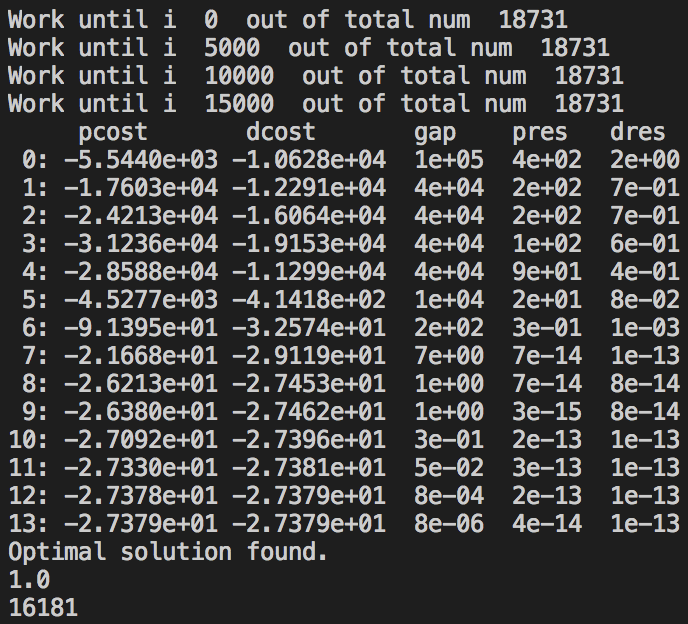
\includegraphics[width=0.5\linewidth]{Linear.png}
\end{figure}

\section{Kernel SVM}

\qquad I applied four different kernels for kernel SVM, linear, Gaussian, Laplace and Polynominal. The results are shown below. Here are linear and Gaussian.

\begin{figure*}[h]
\centering
\subfigure{
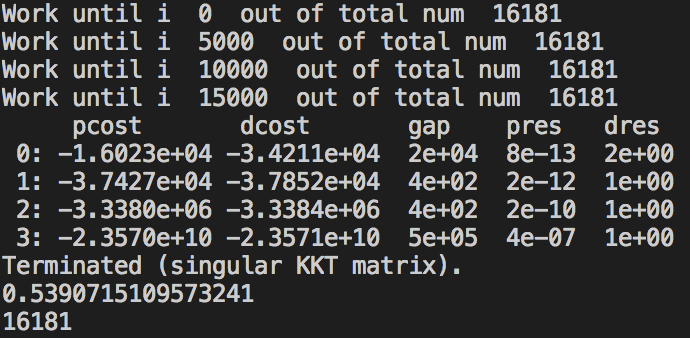
\includegraphics[width=0.4\linewidth]{Linear_dataset_2.png}}
\subfigure{
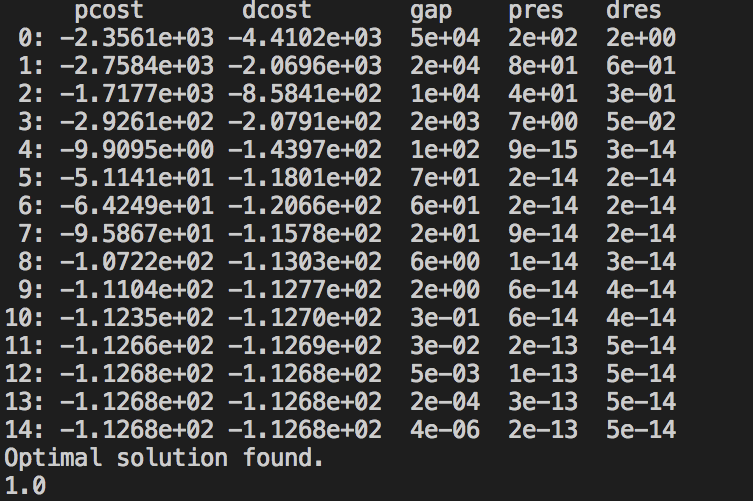
\includegraphics[width=0.4\linewidth]{Gaussian.png}}
\end{figure*}

\newpage

And Laplace and Polynominal as follow.



The error rate of linear kernel is very high, because the data is not linearly separatable.

\section{Soft Margin SVM}

\qquad By applying the Soft Margin SVM from the manual onto our model, and train via the data set 3, we get the following result, with $C = 0.1$.

\begin{figure*}[h]
\centering
\subfigure{
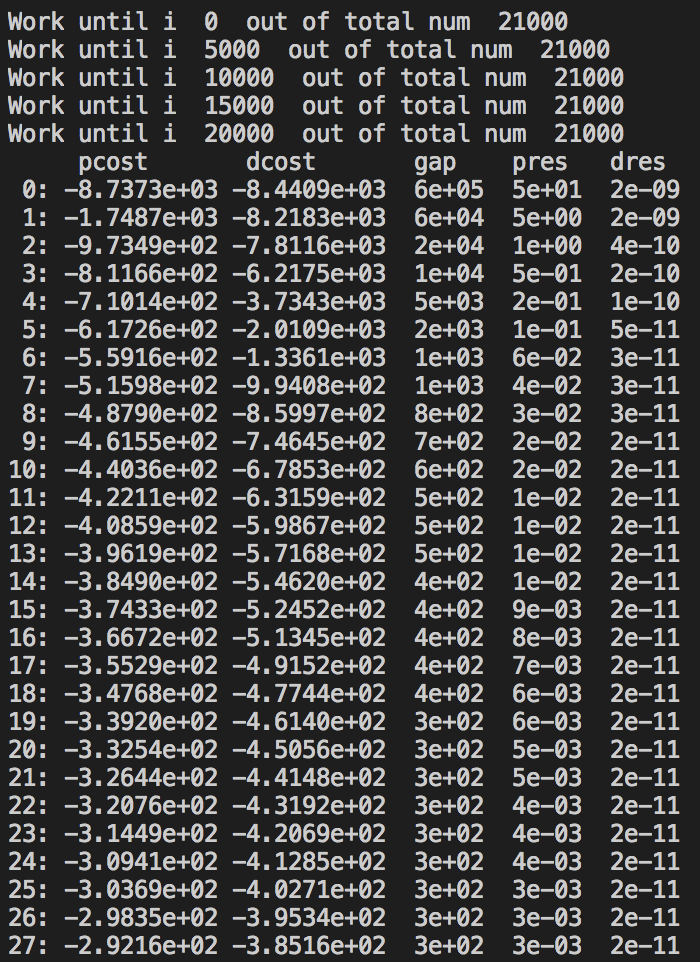
\includegraphics[width=0.4\linewidth]{Soft_1.png}}
\subfigure{
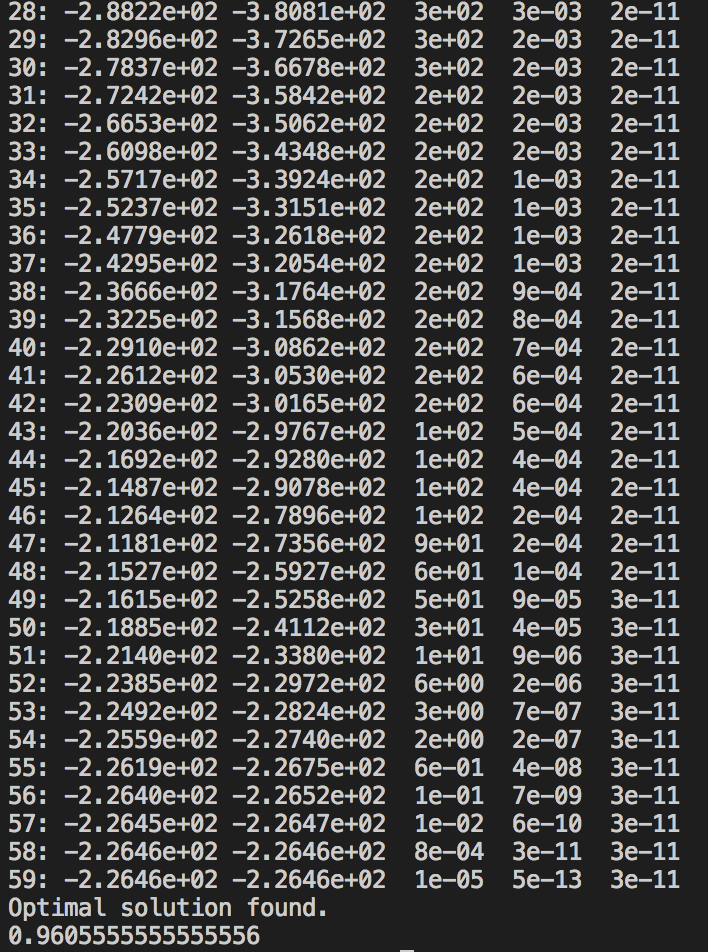
\includegraphics[width=0.4\linewidth]{Soft_2.png}}
\end{figure*}

The error rate is very low, but the training process is so tedious, where I let it run before I go to bed, and it remained unfinished after I got up next morning, and it took the convex optimizor a long time to get the optimal value. So we need to introduce some other ways to solve this problem. You can view the code in class SoftMargin.

\section{ISVM and LSVM}

\qquad I also implemented the LSVM, which is an update of ISVM, and other than the functions provided by the Soft Margin SVM, LSVM and ISVM can support online training, which significantly reduce the resourses needed to train a SVM model.

For ISVM, we suppose that with some data, we trained a SVM model, and get the support vectors. We record the support vectors from the current model, and with the external data coming in, we train the model again with the whole external data as well as the current support vectors. Since with a small amount of support vectors, the whole image can thus be discribed, then the vectors which are not support vectors can be thrown away. We only care about the support vectors.

However, there are some concerns for the ISVM, since both the newly added vectors and the former support vectors are considered of same weight, the support vectors are more likely to be ignored when the external data has a great population. So we multiple an "L" on the former supporting vectors, making it LSVM.

The following function shows the lose function of LSVM with a Soft Margin.

$$
min(w, b, \xi)\quad \frac{1}{2}||w||^2 + C(\Sigma_{i\in I}\xi_i + L \cdot \Sigma_{i\in S}\xi_i)
$$

with L

$$
L = \frac{\# examples}{\# SVs}
$$

By this way, if we split a large data set into small data sets with size $O(1)$, then the total time needed is $O(n)$, but calculating the Kernel Matrix for a data set with size n is already $O(n^2)$, so for large data set, using this method can significantly reduce the time and memory needed for training the model.

We test the method with data set 3, the result is shown below.

\begin{figure}[H]
\centering
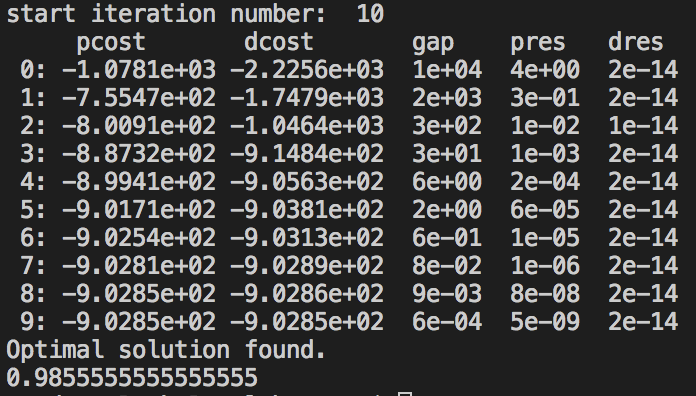
\includegraphics[width=0.5\linewidth]{ISVM.png}
\end{figure}

The error rate is even lower than the Soft Margin SVM. See the code in class ISVM.
\section{Reference}

\begin{enumerate}
\item VE445 Lab 1 Manual
\item Wikipedia Page for SVM \\\url{https://en.m.wikipedia.org/wiki/Support-vector_machine}
\end{enumerate}

\end{document}